\documentclass{article}

\usepackage[left=100pt,right=100pt]{geometry}
\usepackage[round]{natbib}
\usepackage[french]{babel}
\usepackage[utf8]{inputenc}
\usepackage[T1]{fontenc}
\usepackage{float}
\usepackage{graphicx}
\usepackage{multicol}
\usepackage{caption}
\usepackage{subcaption}
\usepackage{mathtools}
\usepackage{afterpage}
\usepackage[normalem]{ulem}
\usepackage{listings}
\usepackage{xcolor}
\usepackage{hyperref}

% Pour l'ajout de Watermark
\usepackage[printwatermark]{xwatermark}
\usepackage{lipsum}
% \newwatermark[allpages,color=gray!20,angle=45,scale=3,xpos=0,ypos=0]{NAME}


% Formattage des hyperliens
\hypersetup{
    colorlinks=true,
    linkcolor=black,
    filecolor=black,
    urlcolor=black,
    citecolor=black
}
\urlstyle{same}

% Change la mise en page des segments de codes
\definecolor{codegreen}{rgb}{0,0.6,0}
\definecolor{codegray}{rgb}{0.2,0.2,0.2}
\definecolor{codepurple}{rgb}{0.58,0,0.82}
\definecolor{backcolour}{rgb}{0.95,0.95,0.95}
\lstdefinestyle{mystyle}{
    backgroundcolor=\color{backcolour},
    commentstyle=\color{codegreen},
    keywordstyle=\color{magenta},
    numberstyle=\tiny\color{codegray},
    stringstyle=\color{codepurple},
    basicstyle=\ttfamily\footnotesize,
    breakatwhitespace=false,
    breaklines=true,
    captionpos=b,
    keepspaces=true,
    numbers=left,
    numbersep=5pt,
    showspaces=false,
    showstringspaces=false,
    showtabs=false,
    tabsize=4
}
\lstset{style=mystyle}

\renewcommand{\contentsname}{Table des matières}
\renewcommand{\listfigurename}{Table des figures}
\renewcommand{\refname}{Bibliographie}
\renewcommand{\lstlistingname}{Segment de codes}
\renewcommand{\lstlistlistingname}{Table des segments de code}

\bibliographystyle{plainnat}

\setlength\parindent{0pt} % Enleve les indentations dans le document

\title{Laboratoire 3\\
  \large Noise2Noise\\
  \normalsize Durée : 2 séances}
\author{Par Christophe Lamarche}
\date{Mise à jour: \today}


\begin{document}
\maketitle

\section{Description}
L'utilisation de filtre pour retirer du bruit dans un signal est amplement vue dans le curriculum d'ingénierie électrique. Les filtres observés sont statiques et cernent des fréquences particulières. Pour le traitement et la réduction de bruit à l'intérieur d'images, l'ÉTS offre le cours ELE747 \citep{ELE747}.

\bigbreak
Ce laboratoire vise à initier l'étudiant à interpréter des papiers scientifiques pour reproduire des modèles neuronaux et d'introduire l'utilisation de banques de données publiques.

\subsection{Exposé du problème}
Le but de ce laboratoire est de réduire le bruit d'images en utilisant les technologies mises de l'avant par le papier de recherche \textbf{Noise2Noise} \citep{Noise2Noise}. L'équipe du laboratoire de recherches chez Nvidia a utilisé l'architecture Unet \citep{Unet} afin de retirer le bruit d'images. La particularité de leur méthode vient à utiliser uniquement des données bruitées pour entraîner leur modèle \citep{Noise2Noise}.

\bigbreak
L'utilisation de données bruitées offre la possibilité d’entraîner des modèles pour des situations où la récolte de données sans bruit est difficile.

\section{Conception de Noise2Noise}
\subsection{Base de données}
Plusieurs services existent pour trouver et télécharger des bases de données. La compagnie \textbf{Google} offre un moteur de recherche pour les bases de données avec leur site web :
\smallbreak
\begin{center}
  \href{https://datasetsearch.research.google.com/}{https://datasetsearch.research.google.com/}
\end{center}

\begin{figure}[H]
  \centering
  
\includegraphics[width=0.5\columnwidth]{figures/googledataset}
  \caption{Moteur de recherche pour des bases de données}
  \label{fig:googleds}
\end{figure}

\bigbreak
À l'aide de ce site, il est possible de rechercher notre base de données d'images.
\bigbreak
Dans notre cas, nous cherchons à télécharger plusieurs images. Par exemple, avec les mots clés \textbf{images} et \textbf{flickr}, un lien vers le site \textbf{Kaggle} est offert.

\bigbreak
\begin{figure}[H]
  \centering
  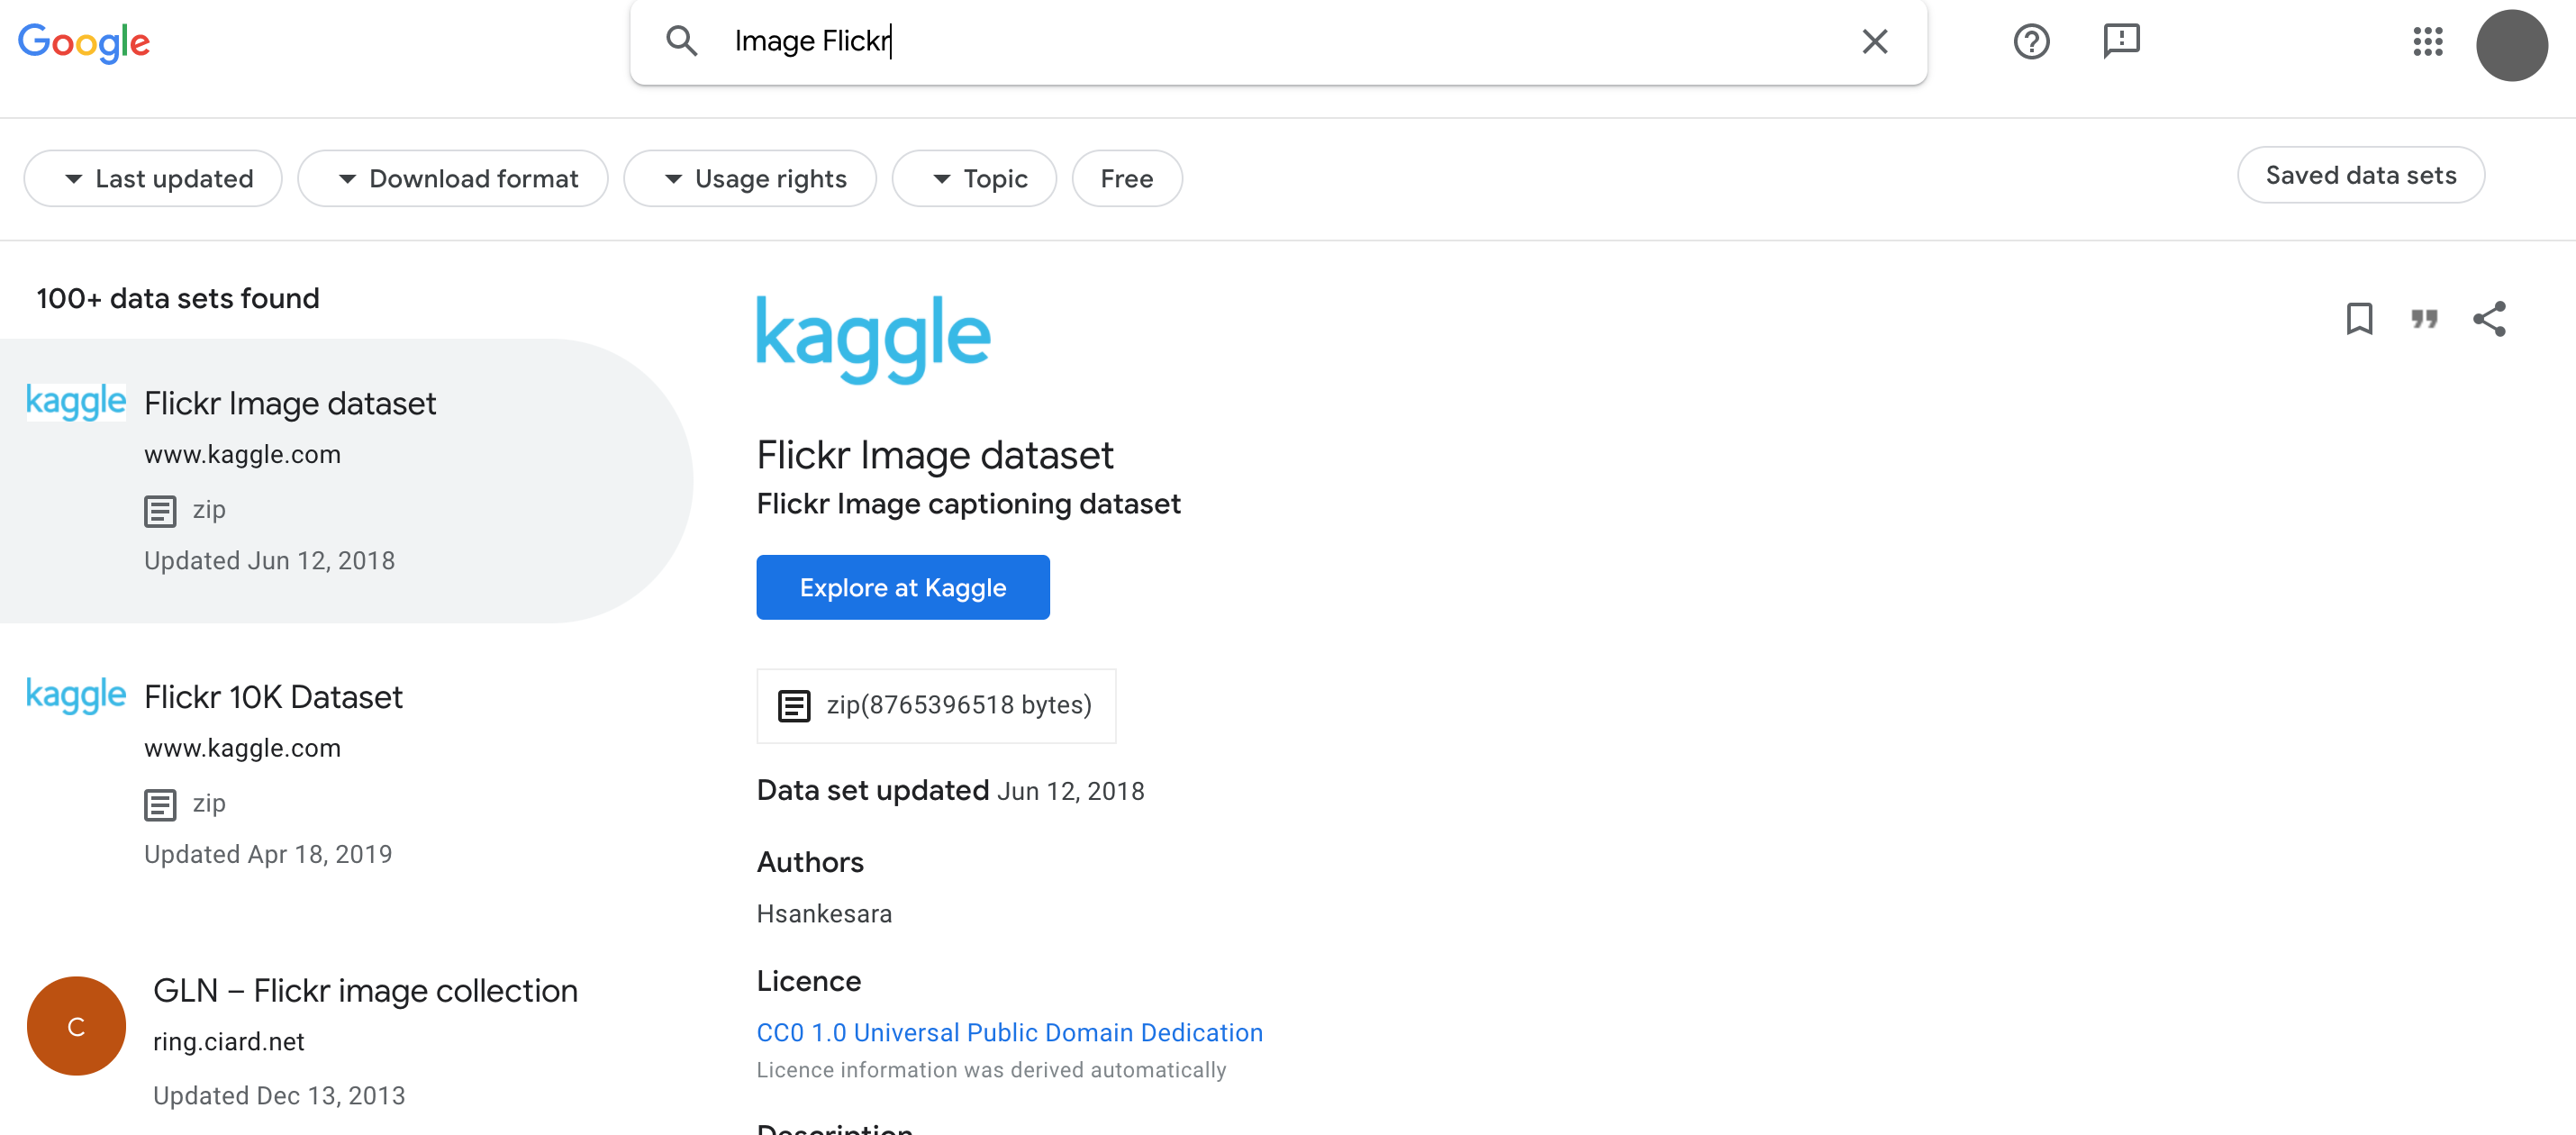
\includegraphics[width=0.5\columnwidth]{figures/flickr_result}
  \caption{Résultats pour les mots ``Image Flickr''}
  \label{fig:image_flickr}
\end{figure}

\bigbreak
\textbf{Kaggle} est un site offrant des services pour la communauté d'analyste de données (\textit{data analyst}) et de scientifiques en apprentissage machine (\textit{machine learning practitioners}). Les utilisateurs du site peuvent accéder et offrir des bases de données à la communauté. En plus, de donner accès à des \textit{notebooks} tels que ceux produits avec \textit{Google Colaboratory}, \textbf{Kaggle} offre aux utilisateurs de participer à des cours en ligne et des compétitions d'analyse de données.

\subsubsection{Accéder à la clé de l'API de Kaggle}
Les \textit{notebooks} de \textit{Google Colaboratory} sont configurés pour interfacer avec l'API de \textbf{Kaggle}. Pour ce faire, il est nécessaire de télécharger notre clé de l'API pour avoir accès aux fonctionnalités.

\bigbreak
Sur le site web de \textbf{Kaggle}, connectez-vous ou inscrivez-vous pour un compte de Kaggle. Les comptes \textbf{Kaggle} sont gratuits et il est possible d'en créer un directement à l'aide d'un compte \textit{Google} ou bien un compte \textit{Facebook}.

\bigbreak
Pour créer un compte, cliquer le bouton ``\textit{Register}'' dans le coin supérieeur droit de la page d'accueil de \textbf{Kaggle}.

\bigbreak
\begin{figure}[H]
  \centering
  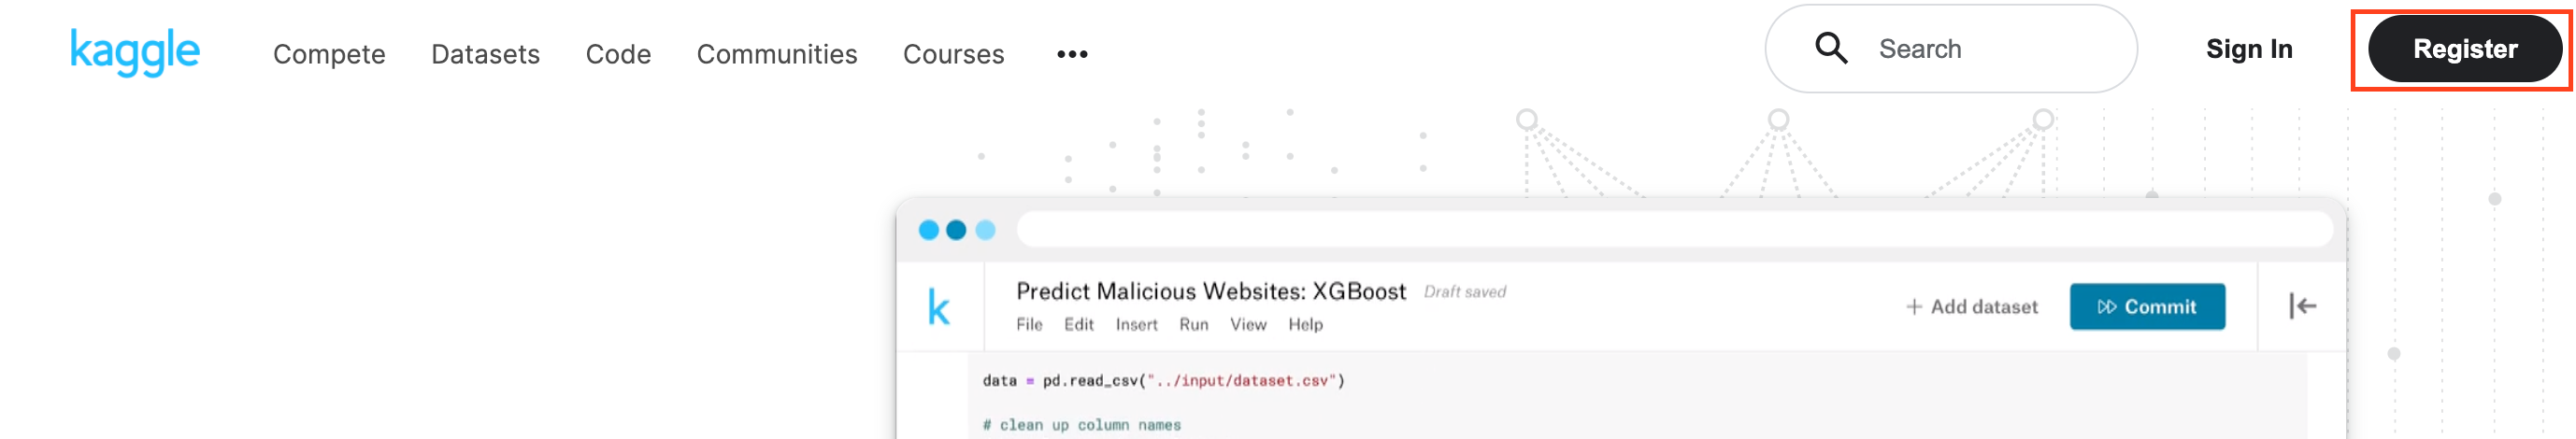
\includegraphics[width=0.5\columnwidth]{figures/kagglesignin}
  \caption{Création d'un compte sur Kaggle}
  \label{fig:kaggle_signin}
\end{figure}

\bigbreak
\begin{figure}[H]
  \centering
  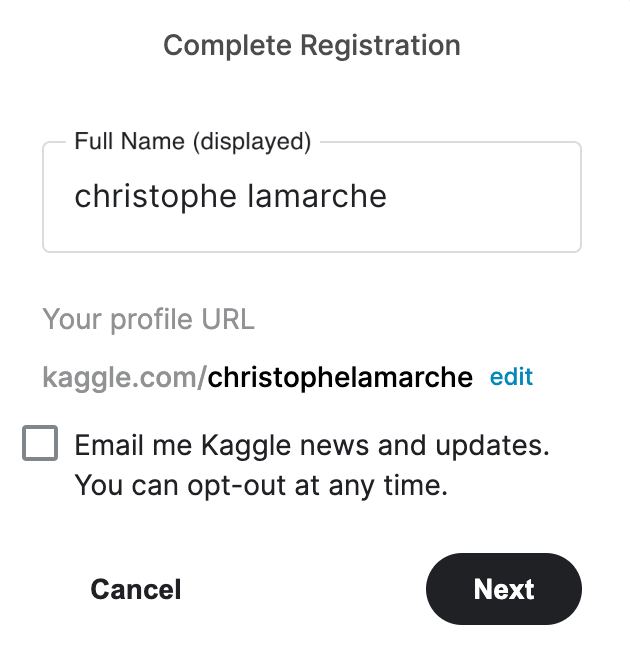
\includegraphics[width=0.5\columnwidth]{figures/create_account}
  \caption{Choisir le nom de l'utilisateur}
  \label{fig:create_account}
\end{figure}


\bigbreak
À la suite que le compte soit fait, dirigez-vous vers les paramètres de compte situés sous la photo de profil.

\bigbreak
\begin{figure}[H]
  \centering
  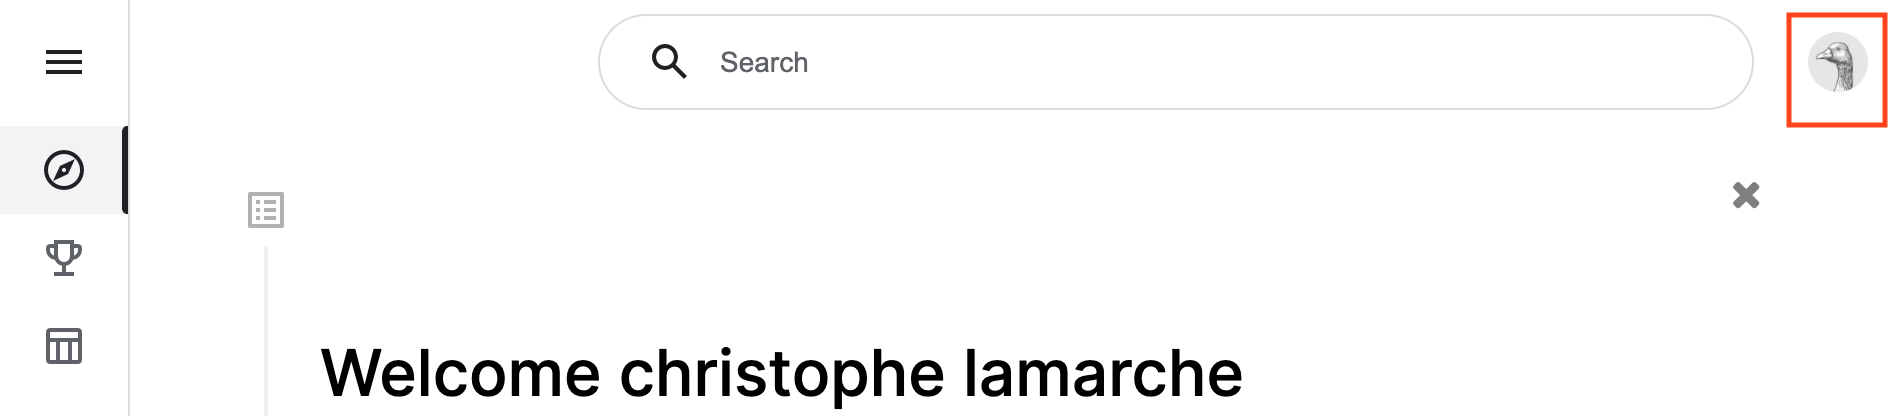
\includegraphics[width=0.5\columnwidth]{figures/click_account}
  \caption{Accéder les options de compte}
  \label{fig:account_options}
\end{figure}

\bigbreak
\begin{figure}[H]
  \centering
  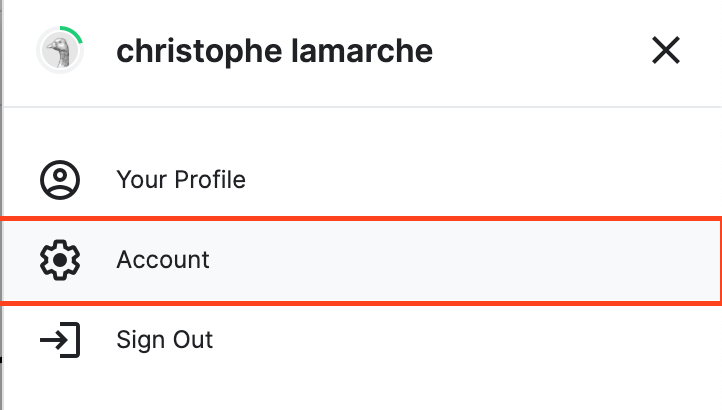
\includegraphics[width=0.5\columnwidth]{figures/account_settings.png}
  \caption{Accéder aux paramètres de compte}
  \label{fig:account_settings}
\end{figure}

\bigbreak
Dans les paramètres de comptes, sous l'onglet comptes, déplacez-vous vers la section \textit{API} et cliquez l'option ``créer une clé API''. Le fichier ``kaggle.json'' se téléchargera. Ce fichier contient la clé d'API pour travailler avec \textbf{Kaggle} à partir de Google Colaboratory et de la ligne de commande (\textit{command line}). \textbf{Ce fichier devrait rester privé}. Afin d'être facilement accessible et privé, déposez ce document à l'intérieur de votre \textit{Google Drive} sous un fichier n'ayant pas été partagé à d'autres utilisateurs.

\subsubsection{Utilisation de l'API}
Dans un nouveau \textit{Notebook}, démarrer une cellule de code et copier le segment de code suivant (Segment de code \ref{code:mount_drive} et \ref{code:download_ds}).

\begin{lstlisting}[language=Python, caption={Connecter le notebook avec Google Drive}, label={code:mount_drive}]
from google.colab import drive
drive.mount('/content/drive')
\end{lstlisting}

\bigbreak
\begin{lstlisting}[language=Python, caption={Télécharger la base de données avec Kaggle}, label={code:download_ds}]
# Mettre la cle API accessible pour le SDK de Kaggle
!kaggle -v &> ./file.tmp && rm ./file.tmp
!cp $chemin_de_la_cle_API$ /root/.kaggle/kaggle.json
!chmod 600 /root/.kaggle/kaggle.json

# Telecharger la base de donnees
!kaggle datasets download $nom-de-lutilisateur/nom-de-la-base-de-donnees$
# Decompresser les fichiers
!unzip -o $nom-de-la-base-de-donnees.*$
# Supprimer le fichier compresse
!rm ./*.zip
\end{lstlisting}

\bigbreak
\textbf{Dans le segment de code \ref{code:download_ds}, il est nécessaire de remplacer les informations entre les \$\$}. La première information à inscrire est le chemin de la clé de l'API. Il est facile d'obtenir le chemin en sélectionnant le fichier dans le menu des fichiers.

\bigbreak
\begin{figure}[H]
  \centering
  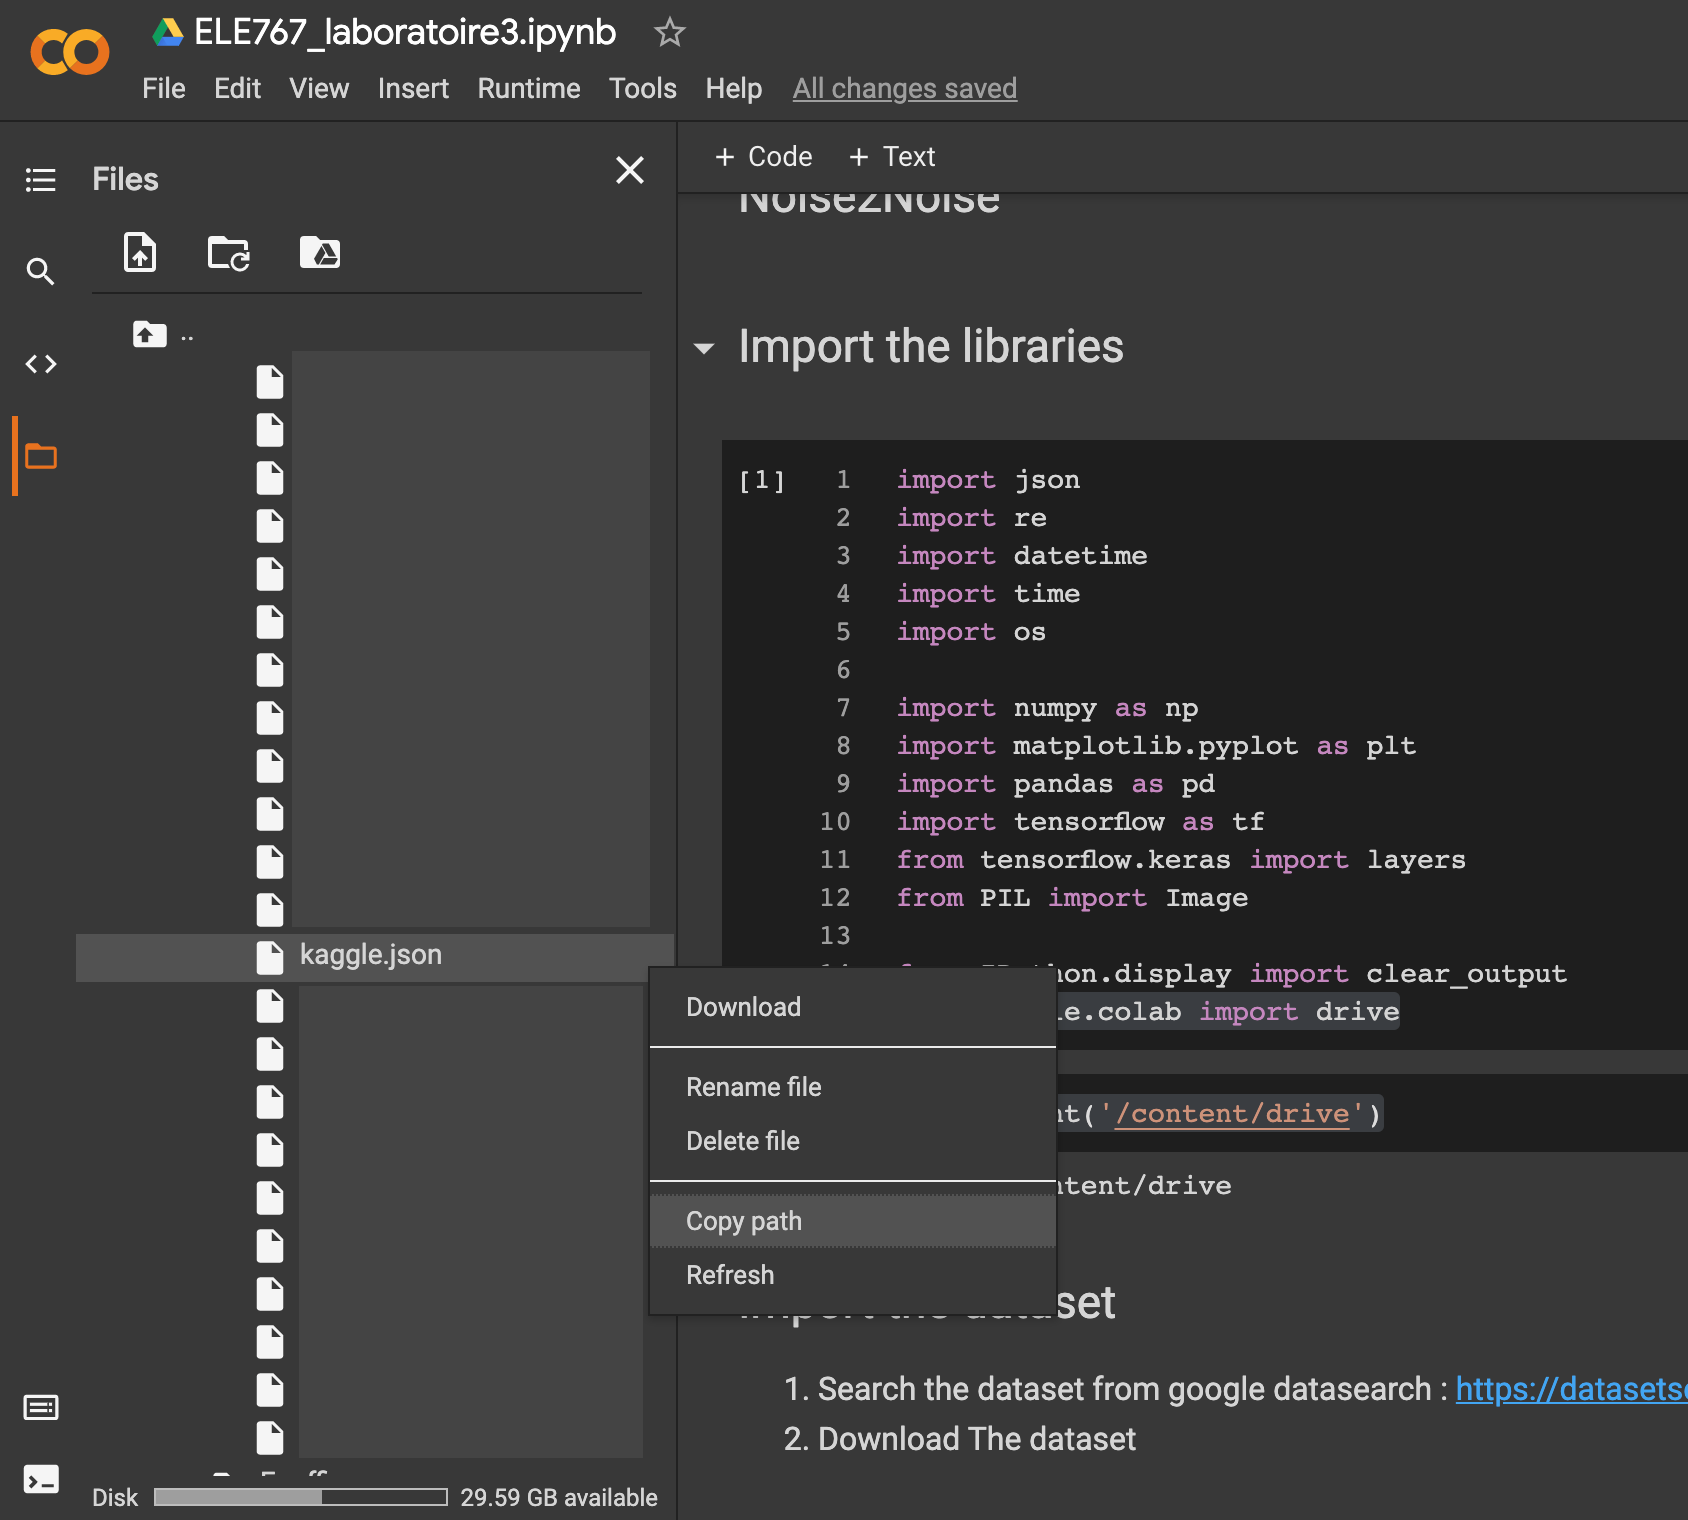
\includegraphics[width=0.5\columnwidth]{figures/copy_path}
  \caption{Copier le chemin de la clé de l'API}
  \label{fig:copy_path}
\end{figure}

\bigbreak
Le chemin de la clé de l'API offert par le menu des fichiers doit être modifié afin d'être inséré dans la commande du segment de code \ref{code:download_ds}. Pour ce faire, les espaces `` '' par une barre oblique inverse jointe d'un espace ``\textbackslash{} ''.

\bigbreak
\textit{Note: Dans le segment de code \ref{code:download_ds}, les lignes commençant par un point d'exclamation ``!'' correspondent à des commandes de terminal.}

\subsubsection{Lecture d'images}
Pour lire les images, nous allons utiliser la librairie ``Pillow (PIL)''. Pour lire les images, nous importons le module ``Image'' de la librairie ``PIL''.

\bigbreak
\begin{lstlisting}[language=Python, caption={Ouverture d'une image avec PIL}, label={code:open_image}]
from PIL import Image
image = Image.open(chemin_image)

# Transformer l'image en matrice
import numpy as np
m_image = np.array(image)
\end{lstlisting}

\subsubsection{Concaténer plusieurs matrices d'images}
La librairie \textit{Numpy} offre la méthode ``numpy.concatenate'' pour joindre plusieurs matrices. Dans notre cas, nous voulons que les images soient accessibles en indexant une matrice. Alors, nous privilégions cette méthode à la méthode ``numpy.stack''.

\bigbreak
\begin{lstlisting}[language=Python, caption={Exemple d'utilisation de la méthode \textit{numpy.concatenate}}, label={code:concatenate}]
import numpy as np

# Creer les matrices a concatener
a = np.random.random((256,256,3))
b = np.random.random((256,256,3))

# Mauvaise concatenation pour notre situation
c = np.concatenate([a,b])
print(c.shape) # >> (512,256,3)

# Bonne concatenation pour notre situation
c = np.concatenate([a.reshape((1,*a.shape)),b.reshape((1,*b.shape))])
print(c.shape) # >> (2,256,256,3)
c = np.concatenate([c,b.reshape((1,*b.shape))])
print(c.shape) # >> (3,256,256,3)
\end{lstlisting}

\subsection{Lecture et interprétation du papier scientifique}
Afin de reproduire le modèle \textit{Noise2Noise} \citep{Noise2Noise}, il est nécessaire de lire le papier ``\href{https://arxiv.org/pdf/1803.04189.pdf}{Noise2Noise: Learning Image Restoration without Clean Data}''.
\bigbreak
(\textit{https://arxiv.org/pdf/1803.04189.pdf})

\subsubsection{Conception du modèle}
Dans le papier scientifique, les auteurs ont produit un tableau (tableau 2) afin de décrire l'architecture du modèle \citep{Noise2Noise}. L'architecture est bien décrite dans la description du modèle et contient toutes les informations nécessaire pour la conception à l'aide de \textit{Tensorflow}.

\bigbreak
Dans cette description, les variables ``\textit{m}'' et ``\textit{n}'' correspondent aux nombres de dimensions de codage. Dans le cas des images téléchargées, le codage des couleurs est de trois dimensions (RGB).

\bigbreak
\textit{Note : Afin de faciliter la création du modèle, je vous conseille d'utiliser la création de modèles sous la forme du segment de code \ref{code:typemodel} afin de réutiliser les entrées de couche. De plus, les couches ``keras'' à utiliser sont énumérées à la table. \ref{tab:couches} }

\bigbreak
\begin{lstlisting}[language=Python, caption={Création de modèle pour la réutilisation d'entrée de couche}, label={code:typemodel}]
from tensorflow.keras import layers

def model(input)
    x_input = layers.Input(shape=input.shape)
    x_flatten = layers.Flatten()(x_input)
    x = layers.Dense(6)(x_flatten)
    x = layers.Concatenate(axis=-1)([x_flatten, x])
    return tf.keras.Model(x_input, x)
\end{lstlisting}

\bigbreak
\begin{table}[H]
\centering
\begin{tabular}{|c|}
  \hline
  Nom de la couche \\
  \hline
  Input \\
  Conv2D \\
  Concatenate \\
  MaxPool2D \\
  UpSampling2D \\
  \hline
\end{tabular}
\caption{Couches à utiliser pour produire le U-Net}
\label{tab:couches}
\end{table}

\bigbreak
\begin{figure}[H]
  \centering
  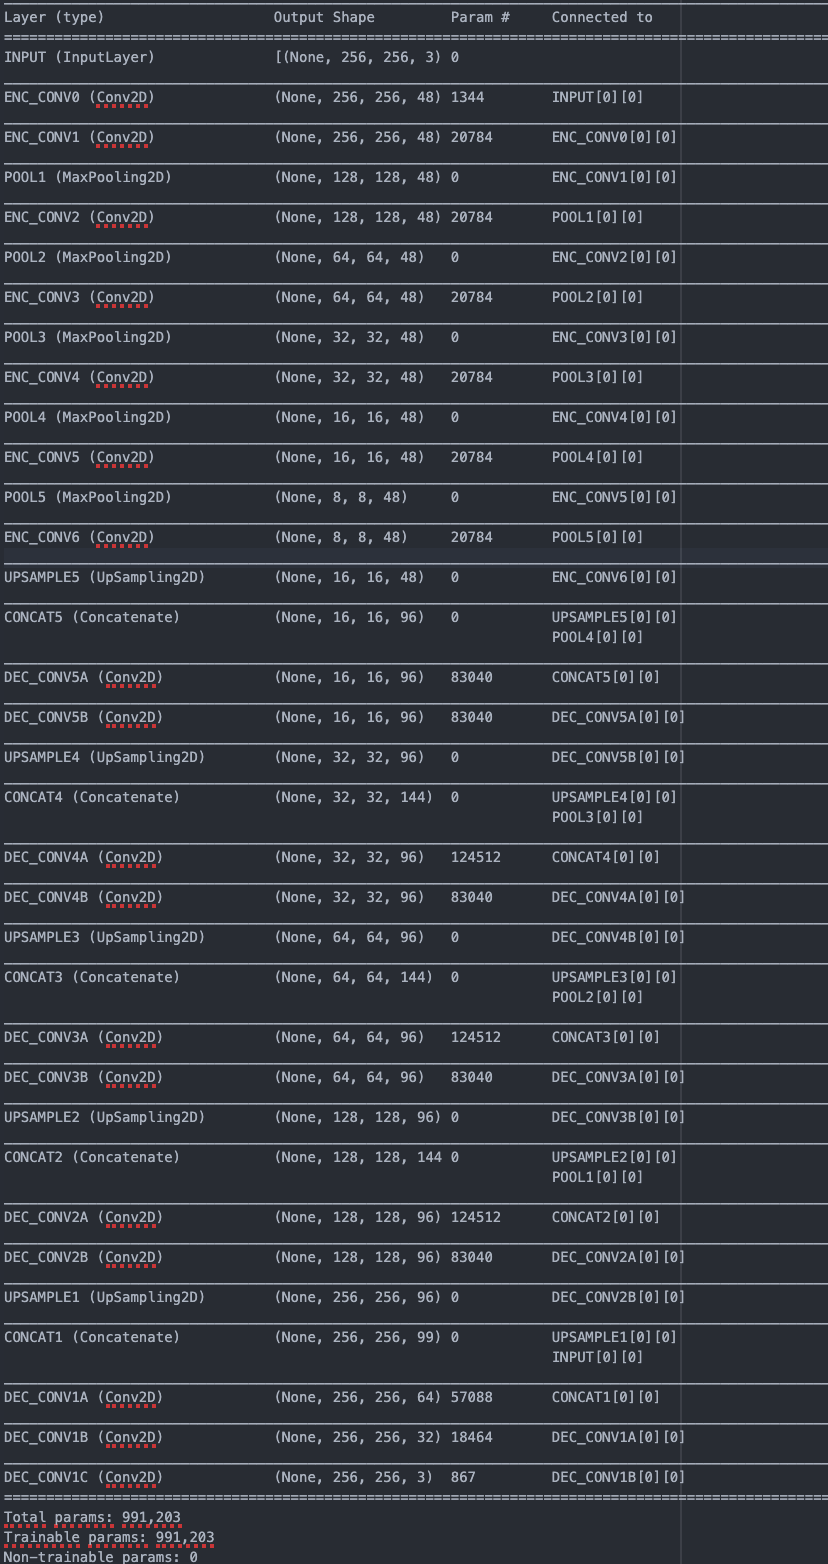
\includegraphics[width=0.5\columnwidth]{figures/summary}
  \caption{Résumé du modèle à produire}
  \label{fig:summary}
\end{figure}

\subsubsection{Ajout de bruit}
Le but du papier \textit{Noise2Noise} \citep{Noise2Noise} est de débruiter les images en entrée. Afin d'obtenir des images davantage bruitées, il est intéressant de produire notre propre bruit. Le type de bruit choisi est intrinsèquement lié au choix de la fonction de perte qui sera utilisée lors de l'entraînement.

\bigbreak
Le choix du type de bruit et de la fonction de perte est votre décision. Basé vous sur le papier \textit{Noise2Noise} \citep{Noise2Noise} pour aider dans votre décision.

\bigbreak
Le bruit consiste à l'ajout de valeur aléatoire au signal. Afin de produire des valeurs selon une distribution normale, la librairie \textit{numpy} offre la méthode ``\textbf{randn}'' sous le module ``\textbf{random}''. Tandisque pour la production de bruit selon une distribution uniforme, la librairie \textit{numpy} offre la méthode ``\textbf{random}'' et ``\textbf{randint}'' sous le module ``\textbf{random}'' dépendamment de la situation d'utilisation.

\subsection{Entraînement du modèle}
Avec les connaissances acquises lors des deux derniers laboratoires, nous allons faire l'entraînement du modèle. L'important dans ce laboratoire sont de bien reproduire les méthodes du papier \textit{Noise2Noise} \citep{Noise2Noise}.

\bigbreak
Dans le cadre du laboratoire, vous devez utiliser la bonne fonction de perte (\textit{loss function}) selon le type du bruit qui a été ajouté aux images.

\bigbreak
L'idée principale derrière \textit{Noise2Noise} est l'utilisation de données bruitées comme données cibles. Le principe est que dans une le cas où l'entraînement est fait sur plusieurs données bruitées différemment, le réseau de neurones apprendra une représentation moyenne du bruit similaire aux images non bruitées.

\subsection{Performance du réseau débruiteur}
Afin de déterminer la performance du réseau pour débruiter une image, nous pouvons utiliser l'équation de ``\textit{Peak Signal-to-Noise Ratio} (PSNR)'' \citep{PSNRWiki}.

$$PSNR = 20 * log(\frac{MAX(Image_{originale})}{MSE(Image_{originale},Image_{Bruitee})})$$

\bigbreak
Cette équation offre une valeur élevée lorsque le bruit est faible et inversement, une valeur basse lorsque le bruit est élevé grâce au \textit{MSE} au dénominateur. De cette manière, en utilisant le résultat du réseau de neurones sur une image précise, il est possible de comparer les performances durant l'entraînement.

\section{À mettre dans le rapport} % Document à remettre
Avec le rapport, il faut remettre le notebook (`.ipynb') et le dossier ``modeles''
\medbreak

Pour télécharger le fichier du notebook, cliquez l'option ``Télécharger .ipynb'' (\textit{``Download .ipynb''}) sous l'onglet fichier.

\begin{figure}[H]
  \centering
  \fbox{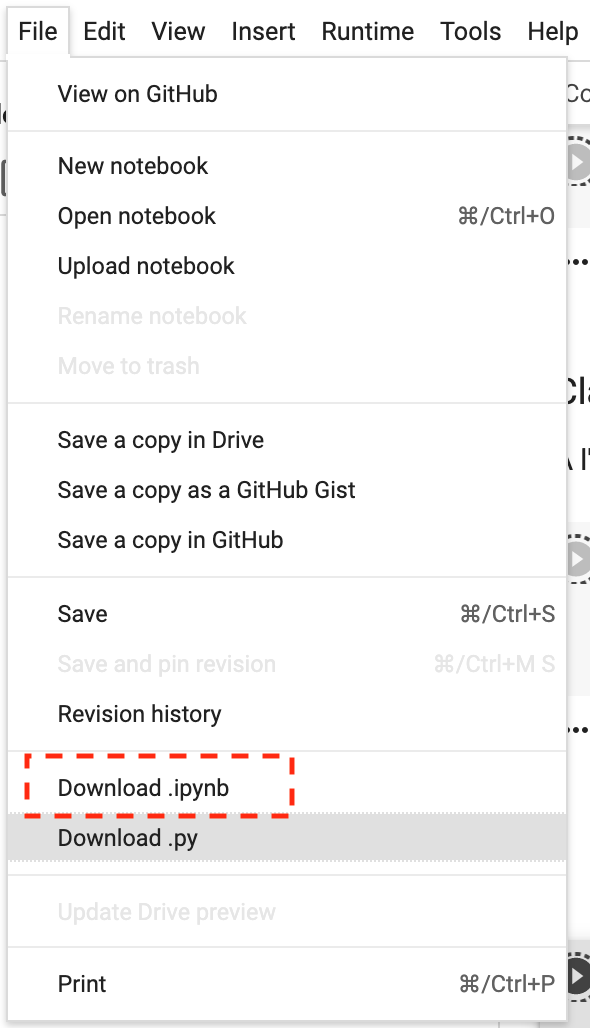
\includegraphics[height=0.75\linewidth]{figures/downloadipynb}}
  \caption{Télécharger le notebook}
  \label{fig:downloadipynb}
\end{figure}
\medbreak
Afin de télécharger le dossier ``modeles'', il faut le compresser auparavant. Pour se faire, ouvrer une nouvelle cellule de code et insérer la commande ci-dessous.

\begin{lstlisting}[language=Python, caption={Compresser un fichier sur une session}, label={code:zip}]
!zip -r modeles.zip ./modeles
\end{lstlisting}
\smallbreak
\textit{Faites attention au point d'exclamation [!] au début de la commande}

\medbreak
Par la suite, il est possible de télécharger en se dirigeant sur l'icône de fichier dans la barre de gauche du notebook tel que représenté dans la figure \ref{fig:downloadzip}.
\begin{figure}[H]
  \centering
  \fbox{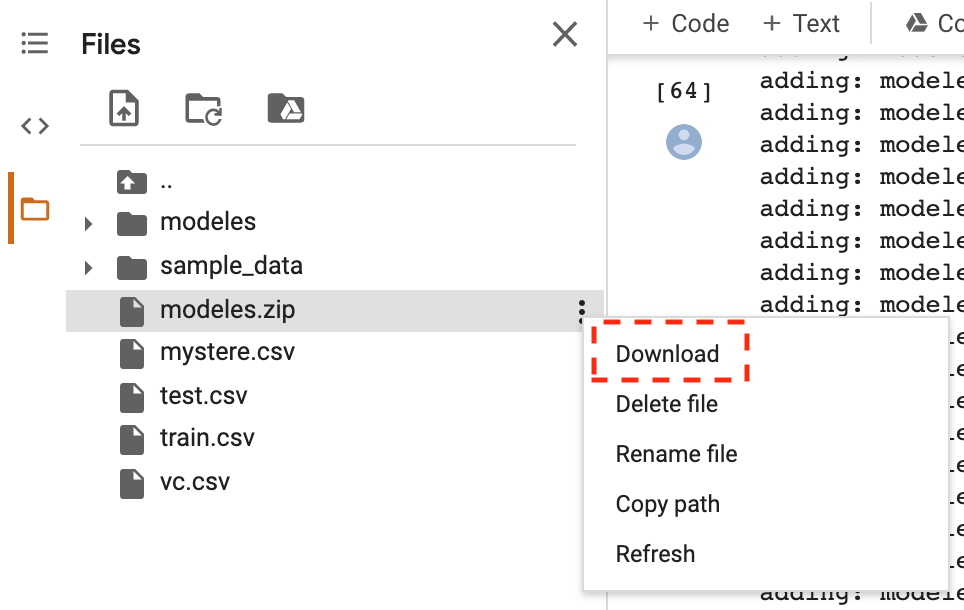
\includegraphics[width=0.75\linewidth]{figures/downloadzip}}
  \caption{Télécharger le dossier compressé}
  \label{fig:downloadzip}
\end{figure}

\begin{table}[H]
  \caption{Contenu du rapport}
  \label{tab:remettre}
  \centering
  \begin{tabular}{|l|l|l|c|}
    \hline
    Section & Taille minimum & Pondération \\
    \hline
    Introduction & 3 lignes & 5\%\\
    Théorie & 5 lignes & 20\%\\
    Résultats & 5 lignes & 40\%\\
    Conclusion & 5 lignes & 35\%\\
    \hline
  \end{tabular}
\end{table}

\subsection{Description des sections}
\subsubsection{Introduction}
Dans l'introduction, il faut décrire le but du laboratoire et de résumer la procédure du laboratoire.

\subsubsection{Théorie}
Dans la section théorique, il est nécessaire d'expliquer les théories et les concepts qui sont mis de l'avant par le laboratoire.

\subsection{Résultats}
La section des résultats doit inclure les graphiques, les tableaux obtenus durant le laboratoire. Il est nécessaire d'inclure une figure décrivant l'entrainement pour chaque modèle. De plus, il est nécessaire d'expliquer le résultat observé à l'intérieur de la figure.

\subsubsection{Conclusion}
Finalement, la conclusion doit contenir un simple retour sur le but, une évaluation des résultats et une ouverture sur l'amélioration du laboratoire.

\bibliography{references}

\end{document}
